\chapter{C++}

\section{Variables}

\begin{verbatim}
    int: integers                   // 4 bytes
    double: floating-point numbers  // double 8 bytes
    char: individual characters     // 1 byte
    float:                          // 4 bytes
    long:                           // 4 or 8 bytes (platform dependent)
    long long:                      // 8 bytes
    bool: true/false                // 1 byte

    // use sizeof for size
bool flag;
std::cout << "Size of int: " << sizeof(numInt); 

\end{verbatim}


\section{Touples}


\section{Enums}

\begin{verbatim}
enum class Day {
    Monday,
    Tuesday,
    Wednesday,
};

int main() {
    Day today = Day::Tuesday;

    if (today == Day::Saturday || today == Day::Wednesday) {
    } else {}

    return 0;
}

enum Color {
    Red,
    Green,
    Blue
};

void printColor(Color color) {
    switch (color) {
        case Red:
            break;
        case Green: // ...
            break;
        case Blue: // ...
            break;
    }
}

int main() {
    Color favoriteColor = Color::Green;
    printColor(favoriteColor);

    return 0;
}
\end{verbatim}

\subsection{Enum with Array Mapping}

\begin{verbatim}
enum class Fruit {
    Apple,
    Banana,
    Orange
};

const std::array<std::string, 3> fruitNames = {
    "Apple",
    "Banana",
    "Orange"
}

const std::string fruitNames[] = { // c-style array
                                   // size by initializer
    "Apple",
    "Banana",
    "Orange"
};

int main() {
    Fruit selectedFruit = Fruit::Banana;
    int fruitIndex = static_cast<int>(selectedFruit);

    std::cout << "Selected fruit: " << fruitNames[fruitIndex] << std::endl;

    return 0;
}
\end{verbatim}

\subsection{Enum with Vector Mapping}

\begin{verbatim}
enum class Month {
    January,
    February,
    March // ...
};

const std::vector<std::string> monthNames = {
    "January",
    "February",
    "March" // ... 
};

int main() {
    Month currentMonth = Month::May;
    int monthIndex = static_cast<int>(currentMonth);

    std::cout << "Current month: " << monthNames[monthIndex] << std::endl;

    return 0;
}
\end{verbatim}


\section{Arrays}

A fixed-size stack-based container. Having the size type information gives more optimization oppotunities.

\begin{verbatim}
#include <array> // c++ 11
    std::array<char, 128> second = {'H', 'e', 'l'} // from library
                            // fixed size of 128
                            // has .begin(), .end(), .at(), .size() 

    sint arr[] = {1, 2, 3}; // c-style array 
                            // size determined by initializer's list
                            // fixed at compile-time 

std::array<Type, Size> data

#include <numeric>
#include <array>

template<typename Value_Type>
std::array<Value_Type, 3> get_data(const Value_Type &v1, const Value_type &v2,
                                   const Value_type &v3)
{
    std::array<Value_Type 3> data;
    data[0] = v1;
    data[1] = v2;
    data[2] = v3;
    return data;
}

// no dynamic allocation, 
// win-win scenario with knowing the size of the data struture at compile time.

template<typename> VT> // takes 3 parameters
std::array<VT, 3> get_data(const VT &v1, const VT &v2, const VT &v3)
{
    return {v1, v2, v3};
}

template<typename> VT> // takes 4 parameters
std::array<VT, 4> get_data(const VT &v1, const VT &v2, const VT &v3, const VT &v4))
{
    return {v1, v2, v3, v4};
}

... 
// If only there was a way to avoid all this code duplication !!!
\end{verbatim}

\subsection{Dynamic Array Allocation}

Achieved using pointers and dynamic memory allocation operators, such as `new` and `delete`. 
While arrays are considered static containers,
dynamic arrays allow you to allocate memory at runtime.

\begin{verbatim}
int size = 5; // desired size of the array
int* dynamicArray = new int[size]; // allocate memory for the array

// Access and modify elements of the dynamic array
dynamicArray[0] = 10;
dynamicArray[1] = 20;
// ...

// Deallocate the memory when it's no longer needed
delete[] dynamicArray;

#include <array>

int main() {
    std::array<int, 3> ar{1,2,3};

    int* dyn_ar = new int[4];

    dyn_ar[0] = 10;
    dyn_ar[1] = 20;
    dyn_ar[2] = 30;
    dyn_ar[3] = 40;
    dyn_ar[4] = 50;
    dyn_ar[5] = 60;
    dyn_ar[6] = 70;

    for (int i = 0; i < 7; i++) {
        std::cout << dyn_ar[i] << " ";
    }
    std::cout << std::endl; // prints 10, 20, 30, 40.. 70.

    delete[] dyn_ar;

    return 1;
}

\end{verbatim}

`new int[size]` dynamically allocates memory. 
`delete[] dynamicArray` deallocates the memory to avoid memory leaks.

Alternatively, using smart pointers or container classes like `std::vector` can help automate memory management
and provide safer alternatives for dynamic arrays.

\section{Vectors}

Vectors are \textbf{dynamic array-like container that can grow or shrink.}

\begin{verbatim}
  std::vector<double> subway_adult; // value is 0.0 is default
  std::vector<double> location(2); // initialize two elements! 
}

std::vector<char> vowels = {'a', 'e', 'i', 'o', 'u'};
std::vector vec{1,2,3}; // now possible! 

int main(int argc, char* argv[]) {
    std::vector<std::string> arguments(argv + 1, argv + argc);

}

#include <vector>

template<typename Value_Type>
std::vector<Value_Type> get_data(const Value_Type &v1, const Value_Type &v2,
                                 const Value_Type &v3)

{
    std::vector<Value_Type> data;
    data.push_back(v1);
    data.push_back(v2);
    data.push_back(v3);
    return data;
}
\end{verbatim}

\section{Size\_t}

\begin{verbatim}
template<typename Value_Type>
struct Data {
    Data(const std::size_t size)
      : data(new Value_Type[size]) // constructor
    {
    }

    ~Data() { delete [] data; }

    Value_Type *data;
};
\end{verbatim}

Size of the dynamically allocated array `data` in the `Data` struct. 
std::size\_t is an unsigned integer type.
specifically designed to represent the size of objects or arrays. 

In the `Data` struct, the constructor takes a `std::size\_t` parameter named `size`,
which specifies the desired size of the `data` array. 
By using `std::size\_t` as the parameter type, 
it ensures that the value provided for `size` is appropriate for representing the size of the array.

Inside the constructor, the `data` member is \textbf{allocated dynamically using `new`}.

The size of the array is specified as the value of `size`, which is of type `std::size\_t`. 
This ensures that the correct amount of memory is allocated for the array based on the given size.

In the destructor, `std::size\_t` is not directly used, but it is common to use `std::size\_t`
for deallocating memory when deleting dynamically allocated arrays, as shown with `delete [] data;`.

This ensures that the memory occupied by the `data` array is properly deallocated.

\subsection{Type mismatch (int vs std::size\_t)}

Size() of containers returns a value of type size\_t, 
an unsigned integral type specifically designed for representing sizes of objects.

Comparing a `size\_t` value with an `int`, causes a mismatch.
Comparing s signed integer with an unsigned value causes UB.

To solve it, either change the type of the loop variable `i` to `size\_t`
or you can cast the container's size to `int` for comparison.

\begin{verbatim}
Option 1: Change the loop variable type to `size_t`:
for (size_t i = 0; i < container.size(); ++i) {
    // ...
}

Option 2: Cast the container's size to `int`:
for (int i = 0; i < static_cast<int>(container.size()); ++i) {
    // ...
}

for (int i = 0; i < container.size(); ++i) {
    // oops mismatched types
}
\end{verbatim}


\subsection{User Input}

\begin{verbatim}
std::cout << "Enter your password: ";
std::cin >> password;

#include <iostream>
#include <string>
#include <cstdlib>

int main() {
    std::string answer;
    std::cout << "Place the output in" << output_dir << "? [y/yes, n/no]: ";
    std::cin >> answer;

    if (answer == "y" || answer == "yes") {
    } else if (answer == "n" || answer == "no") {
    } else {
        std::cout << "Invalid response, exiting";
        std::exit(1) // (failure)
    }
    return 0;
}
\end{verbatim}

\section{Iterators}
\subsection{Conditionals}

\begin{verbatim}
  if (coin == 0) {
  }	else {}
}
\end{verbatim}

\subsection{Switch Statements}

\begin{verbatim}
int main() {
  int number = 9;
  switch(number) {
    case 1 : // ...
      std::cout << "case one";
      break;
    case 2 :
      break;
    default : // ...
      break;
  }
}
\end{verbatim}

\subsection{Loops}

\begin{verbatim}
while (guess != 8) {
  std::cout << "Wrong guess, try again: ";
  std::cin >> guess;
}

for (int i = 0; i < 20; i++)  // incrementing
{}
for (int i = 20; i > 0; i--) // decrementing
{}
\end{verbatim}

\section{Ranges}

\begin{verbatim}
#include <format>
#include <string_view>

void print_map(const auto &map, const std::string_view &key_desc = "key",
                                const std::string_view &value_desc = "value")
{
    const auto print_key_value = [&](const auto &data) { 
        const auto &[key, value] = data;
        std::puts(std::format("{}: '{}' {}: '{}'",
                         key_desc, key, value_desc, value).c_str());
    };

    for_each(map, print_key_value);
}

#include <vector>
#include <ranges>

int main()
{
    std::vector<int> ints{1, 2, 3, 4, 5};
    auto even = [](int i){ return 0 == i % 2; };
    auto square = [](int i){ return i * i; }; // this is a lambda!
                                              // it defines an anonymous function
                                              // on the fly.

    for (int i : ints | std::view::filter(even) | std::view::transform(square)) {
        std::cout << i << ' ';
    }
}
\end{verbatim}

\subsection{Pipes for Ranges}

`|` are operators for composing ranges in C++20.

They chain range adaptors, transforming or filtering operations.
Pipes take the output of one range and passes it as the input to the next range adaptor,
allowing you to compose multiple operations on a range in a concise and readable way.

\begin{verbatim}
auto even = [](int i){ return 0 == i % 2; };
auto square = [](int i){ return i * i; }; // this is a lambda!

for (int i : ints | std::view::filter(even) | std::view::transform(square)) {
    std::cout << i << ' ';
}

`ints`: The input range of integers.
`std::view::filter(even)`: Filters the `ints` range, keeping only the even numbers.
`std::view::transform(square)`: Transforms the filtered range by squaring each element.
`int i : ...`: Iterates over the resulting transformed range and assigns each element to `i`.
`std::cout << i << ' ';`: Prints each element `i` separated by a space.
\end{verbatim}

Note that this code snippet utilizes C++20's Ranges library, which requires a compatible compiler with proper language and library support.

\subsection{Range-Based for Loops}


Iteratore over elements of a container, such as an array, std::vector, or std::list. It doesn't work for forward\_list.


Works with anything that has begin()
and end() members/functions, C-Style arrays and initializer lists.

\begin{verbatim}

for (const auto &element : container) {
    // eliminates both other problems
}

for (int element : first_three_multiples(8)) {
 std::cout << element << "\n";
}
std::string str = "Hello";
for (char character : str) {
    std::cout << character << std::endl;
}

template<typename Map>
void print_map(const Map &map, const std::string &key_desc = "key",
                               const std::string &value_desc = "value")
{
    for (const auto &data : map)
    {
        std::cout << key_desc << ": '" << data_itr->first << "' "
                  << value_desc << ": '" << data_itr->second << "'\n";
    }
}

for (const auto &value : container) {} // for each element in the container

standard c++11

Never mutate the container itself while iterating inside of a ranged-for loop. 
Use clang-tidy's modernize-loop-convert check. Not using auto eases silent mistakes in your code.

template<typename Map>
void print_map(const Map &map, const std::string &key_desc = "key",
                               const std::string &value_desc = "value")
{
    for (const auto &data : map)
    {
        std::cout << key_desc << ": '" << data.first << "' "
                  << value_desc << ": '" << data.second << "'\n";
    }
}

// if only there was some way to make this data.first, data.second nonsense more readable!!
\end{verbatim}

\subsection{Accidental conversions}

\begin{verbatim}
for (const int value : container_of_double) {
    // accidental conversion, possible warning
}
\end{verbatim}

\subsection{Accidental slicing}

\begin{verbatim}
for (const base value : container_of_derived) {
    // accidental silent slicing
}

If container_of_derived holds objects of a derived class. 
Base is the base class.
The loop is iterating over the container and assigning each
derived object to a base object (value) due to object slicing.

Object slicing occurs because the base object can only store
the base class's attributes and behavior. Additional defined 
class attributes will be lost during the assignment or copy.

To avoid accidental slicing, you use pointers or references.

// no problem
for (const auto &value : container) {
    // no possible accidental conversion
}

Using pointers or references ensures that 
the derived objects retain their specific attributes and behavior.

const auto & for non-mutating loops
auto & for mutating loops
auto && 
// only when you have to with weird types like std::vector<bool>,
// or if moving elements out of the container
\end{verbatim}

\subsection{Enable Ranged-Loop Warnings}

\begin{verbatim}
GCC/ Clang?

-Wrange-loop-construct
-Wall // included in -Wall
\end{verbatim}

\section{Functions}

\begin{verbatim}
void eat() {
  std::cout << "nom nom\n";
}

bool even(int num) {
  return ( num % 2 == 0 ? true : false );
  // this should be tested
}
\end{verbatim}

\subsection{Inline Functions (2 meanings)}

The compiler inserts the function’s body on the function call

\begin{verbatim}
inline 
void eat() {
  std::cout << "nom nom\n";
}

// or

// function defined and declared in a single line in a header file
void Cookie::eat() {std::cout << "nom nom\n";}

Without inline in header is slower.

// source
std::string goodnight1(std::string thing1) {
  return "Goodnight, " + thing1 + ".\n";
}
// header
std::string goodnight1(std::string thing1);

With inline in header is faster. 0,004 milliseconds faster.

//inline in header, night.hpp
inline
std::string goodnight1(std::string thing1) {
  return "Goodnight, " + thing1 + ".\n";
}
\end{verbatim}

\subsection{Member Functions}

Functions inside of classes.

\begin{verbatim}
class Musician {
private:
    int instruments;

public:
    // Getter function
    int getMyVariable() const {
        return myVariable;
    }

    // Setter function
    void setMyVariable(int newValue) {
        myVariable = newValue;
    }
};

int main() {
    MyClass obj;
    obj.setMyVariable(42);

    int value = obj.getMyVariable();
    std::cout << "MyVariable value: " << value << std::endl;

    return 0;
}
\end{verbatim}

\subsection{Public}

\begin{verbatim}
class City {
  int population; 
 
public: // accessible outside of the class
  void add_resident() { 
    population++;
  }

private: // private to this class
  bool is_capital;
};

#include <string>

class Song { // header song.hpp
  std::string title;
  std::string artist;

public:
  void add_title(std::string new_title);
  std::string get_title();
  
  void add_artist(std::string new_artist);
  std::string get_artist();
};

#include "song.hpp"

void Song::add_title(std::string new_title) { // song.cpp
  title = new_title; // setters
}

std::string Song::get_title() { // getter
  return title;
}

void Song::add_artist(std::string new_artist) { // setters
  artist = new_artist;
}

std::string Song::get_artist() { // getters
  return artist;
}

#include "city.hpp"
 
class City {
  std::string name; // In header, city.hpp
  int population;
 
public:
  City(std::string new_name, int new_pop);
 
};
 
City::City(std::string new_name, int new_pop) // city.cpp
  : name(new_name), population(new_pop) {} // member initialized to passed values.

City ankara("Ankara", 5445000); // works, in main()

// in Header, in song.hpp
class Song {
  std::string title;
  std::string artist;

public:
  Song(std::string new_title, std::string new_artist); // constructor

  void add_title(std::string new_title);
  std::string get_title();

  void add_artist(std::string new_artist);
  std::string get_artist();
};
                ***
#include "song.hpp"

Song::Song(std::string new_title, std::string new_artist) in main, song.cpp
  : title(new_title), artist(new_artist) {}

void Song::add_title(std::string new_title) {
  title = new_title;
}
std::string Song::get_title() {
  return title;
}

void Song::add_artist(std::string new_artist) {
  artist = new_artist;
}

std::string Song::get_artist() {
  return artist;
}

#include <string> // in header file, song.hpp

class Song {
  std::string title;
  std::string artist;

public:
  Song(std::string new_title, std::string new_artist);

  std::string get_title();
  std::string get_artist();
};
                    ***
#include "song.hpp"

Song::Song(std::string new_title, std::string new_artist) // in main song.cpp
  : title(new_title), artist(new_artist) {}

std::string Song::get_title() {
  return title;
}

std::string Song::get_artist() {
  return artist;
}

#include <iostream> // in main.cpp
#include "song.hpp"

int main() { 
  Song back_to_black("Back to Black", "Amy Winehouse");

  std::cout << back_to_black.get_title() << "\n";
  std::cout << back_to_black.get_artist() << "\n";
}
\end{verbatim}

\subsection{Overloading}

Accepts many types as parameters.

Change behavior based on parameter's type.

\begin{verbatim}
// one must be true
    Each has different type parameters.
    Each has a different number of parameters.
    
// in num.cpp 
// defining
int fancy_number(int num1, int num2) {
  return num1 - num2 + (num1 * num2);
}

int fancy_number(int num1, int num2, int num3) {
  return num1 - num2 - num3 + (num1 * num2 * num3);
} // different number of params.

int fancy_number(double num1, double num2) {
  return num1 - num2 + (num1 * num2);
} // different type of params.
// in num.hpp
// declaring
int fancy_number(int num1, int num2);
int fancy_number(int num1, int num2, int num3);
int fancy_number(double num1, double num2);

\end{verbatim}

\subsection{Parameters}

\begin{verbatim}
void get_emergency_number(std::string emergency_number) {}

#include <iostream>
#include <vector>

struct ComplexType {
    int value;
    std::vector<int> data;
};

void processComplexType(const ComplexType& complexParam) {
    std::cout << "Value: " << complexParam.value << std::endl;
    std::cout << "Data:";
    for (int num : complexParam.data) {
        std::cout << " " << num;
    }
    std::cout << std::endl;
}

int main() {
    ComplexType complexObj;
    complexObj.value = 42;
    complexObj.data = {1, 2, 3, 4, 5};

    processComplexType(complexObj);

    return 0;
}

Many Parameters

double get_tip(double price, double tip, bool total_included) {
    get_tip(0.25, true, 45.50); // will not work. Order matters. 
}

#include <iostream>

void name_x_times(std::string name, int x){
  while (x > 0) {
    std::cout << name << "\n";
    x--;
  }
}
\end{verbatim}

\subsection{Pass-by-value (in a function's params)}

\begin{verbatim}
Yet, we can't modify the value of the arguments.
The variable passed are out of scope.

#include <iostream>

struct ComplexStruct {
    int value1;
    int value2;
};

void modifyValue(int val) {
    val = 100;
}

void modifyStruct(ComplexStruct obj) {
    obj.value1 = 200;
    obj.value2 = 300;
}

int main() {
    int x = 10;

    std::cout << "Before modif: x = " << x << std::endl;  
    // Output: Before modif: x = 10

    modifyValue(x);  // Pass x by value to the modifyValue function

    std::cout << "After modif: x = " << x << std::endl;   
    // Output: After modif: x = 10

    ComplexStruct obj;
    obj.value1 = 50;
    obj.value2 = 60;

    std::cout << "Before modif: obj.value1 = " << obj.value1 << std::endl;  
    // Output: Before modif: obj.value1 = 50
    std::cout << "Before modif: obj.value2 = " << obj.value2 << std::endl;  
    // Output: Before modif: obj.value2 = 60

    modifyStruct(obj);  // Pass obj by value to the modifyStruct function

    std::cout << "After modif: obj.value1 = " << obj.value1 << std::endl;   
    // Output: After modif: obj.value1 = 50
    std::cout << "After modif: obj.value2 = " << obj.value2 << std::endl;   
    // Output: After modif: obj.value2 = 60

    return 0;
}

\end{verbatim}

\subsection{Default Values}

\begin{verbatim}
struct Chapters {
    bool IsToPrint = true;
};

struct Chapters {
    bool IsToPrint;

    Chapters() : IsToPrint(true) {} // with default constructor
};

int main() {
    Chapters c1;
    Chapters c2 = {false}; //  list initialization
                           // works when only one bool in struct

    // c1.IsToPrint will be true
    // c2.IsToPrint will be false

    return 0;
}
\end{verbatim}

\subsection{Default Arguments}

\begin{verbatim}
// Declaration
void intro(std::string name, std::string lang = "C++");

// Definition
void intro(std::string name, std::string lang) {
    std::cout << "my" << name << "is" << lang << '\n';
}
\end{verbatim}

\subsection{Ls Function}

\begin{verbatim}
// C++17 // g++ -std=c++17 myfile.cpp -o output-name

#include <filesystem>
namespace fs = std::filesystem;

int main()
{
    std::string path = "./foo";
    for (const auto &entry : fs::directory_iterator(path))
        std::cout << entry.path() << std::endl; // valid single statement synthax
                                                // If no optional block
                                                // only the statement following
                                                // the loop construct is executed.
}

&entry : fs::directory_iterator(path)
& creates a reference to the elements of the fs::directory_iterator object.

\end{verbatim}

\subsection{Standard Library Functions}
\begin{verbatim}
C++ considers system architecture. 
The libraries are differents as well?

Listing files in a directory is different in both OS.
\end{verbatim}

\subsection{Return Type Deduction for Normal Functions}

Not to be underestimated, this allows
for the creation of powerful higher order function constructs, among other things.

\begin{verbatim}
auto get_thing() {
    struct Thing {}; // creating my own type inside the function 

    return Thing{};
}
\end{verbatim}

\section{Reference}
\subsection{References Variables}

\textbf{A second name for an existing variable}

\begin{verbatim}
int &sonny = songqiao; // Sonny, a reference to songqiao;

\\ Changes to the reference happens to the original.
\\ Aliases cannot be changed to alias something else.

  int soda = 99;
  int &pop = soda;
  pop++; // soda and pop equal at 100

Using a reference (&) instead of making a copy of the elements is more efficient,
especially when dealing with large objects or containers. 

By using a reference, the loop avoids creating a new copy of each element
, reducing unnecessary memory usage and improving performance.

#include <iostream>

struct ComplexStruct {
    int value1;
    int value2;
};

void modifyStruct(ComplexStruct& ref) {
    ref.value1 = 100;
    ref.value2 = 200;
}

int main() {
    int x = 10;
    int& ref1 = x;  // Reference variable ref1 refers to x

    std::cout << "x: " << x << std::endl;        // Output: x: 10
    std::cout << "ref1: " << ref1 << std::endl;  // Output: ref1: 10

    ref1 = 20;  // Modifying ref1 will also modify x

    std::cout << "x: " << x << std::endl;        // Output: x: 20
    std::cout << "ref1: " << ref1 << std::endl;  // Output: ref1: 20

    ComplexStruct obj;
    obj.value1 = 50;
    obj.value2 = 60;
    ComplexStruct& ref2 = obj;  // Reference variable ref2 refers to obj

    std::cout << "obj.value1: " << obj.value1 << std::endl;      // Output: obj.value1: 50
    std::cout << "obj.value2: " << obj.value2 << std::endl;      // Output: obj.value2: 60
    std::cout << "ref2.value1: " << ref2.value1 << std::endl;    // Output: ref2.value1: 50
    std::cout << "ref2.value2: " << ref2.value2 << std::endl;    // Output: ref2.value2: 60

    modifyStruct(ref2);  // Modifying ref2 will also modify obj

    std::cout << "obj.value1: " << obj.value1 << std::endl;      // Output: obj.value1: 100
    std::cout << "obj.value2: " << obj.value2 << std::endl;      // Output: obj.value2: 200
    std::cout << "ref2.value1: " << ref2.value1 << std::endl;    // Output: ref2.value1: 100
    std::cout << "ref2.value2: " << ref2.value2 << std::endl;    // Output: ref2.value2: 200

    return 0;
}

\end{verbatim}
\subsection{Dereference}

Obtain the pointer's pointed value. 

\begin{verbatim}
Declaration? * creates a pointer.
Not a declaration? * is a dereference operator.

int main() {
  int power = 9000;
  int* ptr = &power;
  std::cout << *ptr; // prints 9000
}

int main() {
    int x = 10;
    int* ptr = &x;

    std::cout << "Value of x: " << x << std::endl;            
    // Output: Value of x: 10

    std::cout << "Address of x: " << &x << std::endl;         
    // Output: Address of x: 0x7ffeebdbcbe4

    std::cout << "Value of ptr: " << ptr << std::endl;        
    // Output: Value of ptr: 0x7ffeebdbcbe4

    std::cout << "Dereferenced value of ptr: " << *ptr << std::endl;  
    // Output: Dereferenced value of ptr: 10

    *ptr = 20;  // Dereference ptr and assign a new value

    std::cout << "Modified value of x: " << x << std::endl;    // Output: Modified value of x: 20

    return 0;
}
\end{verbatim}

\subsection{Pass-by-reference (in a funtion's params)}

Now, when called, the function can modify the argument's value.
Avoid making copies of a variable/object for performance reasons.

\begin{verbatim}
//Calling swap_num(), variables a and b's value will be modified
//because they are passed by reference

void swap_num(int &i, int &j) {
  int temp = i;
  i = j;
  j = temp;
}
 
int main() {
  int a = 100;
  int b = 200;
 
  swap_num(a, b);
 
  std::cout << "A is " << a << "\n";
  std::cout << "B is " << b << "\n";
}

WHEN? To MODIFY the arguments’ values.

int triple(int &i) {
  i = i * 3;
  
  return i;
}

int main() {
  int num = 1;
  std::cout << triple(num) << "\n";
}

template<typename T>
void modifyVector(std::vector<T>& vec) {
    for (auto& element : vec) {
        element *= 2;
    }
}

template<typename T>
void printVector(const std::vector<T>& vec) {
    for (const auto& element : vec) {
        std::cout << element << " ";
    }
    std::cout << std::endl;
}

int main() {
    std::vector<int> numbers = {1, 2, 3, 4, 5};

    std::cout << "Original vector: ";
    printVector(numbers);  // Output: Original vector: 1 2 3 4 5

    modifyVector(numbers);

    std::cout << "Modified vector: ";
    printVector(numbers);  // Output: Modified vector: 2 4 6 8 10

    return 0;
}
\end{verbatim}

\subsection{Const Reference}

\begin{verbatim}
int triple(int const &i) { // save computational cost
  return i * 3; // don't make a copy of the argument
}

int square(int const &i) {
  return i * i;
}

int main() {
  int side = 5;
  std::cout << square(side) << "\n";
}
\end{verbatim}

\subsection{Reference Operator}

\begin{verbatim}
int soda = 99; // in a declaration
int &pop = soda; // reference operator
pop++;
\end{verbatim}

\subsection{Address Operator}

Not a declaration? It is an address operator.

\begin{verbatim}
int porcupine = 3; 
std::cout << &porcupine << "\n"; 

// 0x7ffd7caa5b54
\end{verbatim}

\subsection{Boarding References}

\begin{verbatim}
auto get_data(auto && ... params)
{
    return std::array{std::forward<decltype(params)>(params)...};
}

// no unnecessary copies of params, guaranteed copy/move elisions of return value.
\end{verbatim}

This does not make c++ easier to teach, but it allows for high level efficiency. At this point, 
is get\_data() even necessary?

\subsection{Rvalue References}

Difficult to teach, but allows to more accurately reason about the lifetime of objects. C++11.

\subsection{Guaranteed Copy Elision}

Compilers have "always done copy elision on return values but c++17 guarantees it in some situations:

\begin{verbatim}
struct S {
    S() = default;
    S(S&&) = delete;
    S(const S &) = delete;
};

auto s_factory(){
    return S{}; // compiles in C++17, neither a copy nor a move.
}
\end{verbatim}

\section{Pointers}

\begin{verbatim}
// Pointers store a memory address. If possible, avoid pointers!

int* number; // Declaring
double* decimal;
char* character;

int gum = 8;
int* ptr = &gum; // int* [declare a pointer]
                 // ptr [pointer's name]
                 // &gum [store gum's memory address in ptr]

int* number; // Declaration standard
int *number;
int * number; // All Synthaxically valid

Certainly! Here are two complex examples showcasing the use of pointers in C++:

Example 1: Pointer to Pointer
```cpp
#include <iostream>

int main() {
    int value = 5;
    int* ptr = &value;
    int** ptrToPtr = &ptr;

    std::cout << "Value: " << value << std::endl;
    std::cout << "Value via pointer: " << *ptr << std::endl;
    std::cout << "Value via pointer to pointer: " << **ptrToPtr << std::endl;

    return 0;
}
```
In this example, we declare a variable `value` and initialize it with the value 5. We then create a pointer `ptr` that points to the address of `value`. Finally, we create a pointer to a pointer `ptrToPtr` that points to the address of `ptr`. We can access the value of `value` through the pointer `ptr` using the dereference operator `*`, and we can access it through the pointer to pointer `ptrToPtr` using double dereference `**`.

// Dynamic Memory Allocation

int main() {
    int size = 5;
    int* dynamicArray = new int[size];

    for (int i = 0; i < size; ++i) {
        dynamicArray[i] = i + 1;
    }

    std::cout << "Dynamic Array: ";
    for (int i = 0; i < size; ++i) {
        std::cout << dynamicArray[i] << " ";
    }
    std::cout << std::endl;

    delete[] dynamicArray;

    return 0;
}

We allocate dynamic memory for an integer array of size 5 using the `new` keyword.
We then populate the array with values from 1 to 5.
Finally, we print and release the allocated memory using `delete[]` to avoid memory leaks.
\end{verbatim}

\subsection{Null pointers}

\begin{verbatim}
// Ptr to a yet unknown memory address. Dangerous stuff!

int* ptr; // declared, not yet initialized
\end{verbatim}

\subsection{Nullptr - null pointers since C++11}

\begin{verbatim}
int* ptr = nullptr; // type safe pointer with nullptr, replacement for NULL
\end{verbatim}

\section{Classes}

\begin{verbatim}
A C++ class is a user-defined type.

class City {
}; // needs semicolon
\end{verbatim}

\subsection{Class Components}

\begin{verbatim}
Class components are called class members
Attributes and methods are class members

class City {
  int population; // attribute
 
public:
  void add_resident() { // method
    population++;
  }
};
\end{verbatim}

\chapter{Object Lifetime}

\section{Constructors}

\begin{verbatim}
City montreal;
montreal.population = 20000;

montreal.get_population();

class Song { // header file, song.hpp

  std::string title;

public:
  void add_title(std::string new_title);
  std::string get_title();
};

void Song::add_title(std::string new_title) {
  title = new_title; // main file, song.cpp
}

std::string Song::get_title() {
  return title;
}
int main() {
  Song electric_relaxation;
  electric_relaxation.add_title("Electric Relaxation");
  std::cout << electric_relaxation.get_title();
}
\end{verbatim}

\section{Destructors}

\begin{verbatim}
------ city.hpp -------

class City { 
  std::string name;
  int population;
 
public:
  City(std::string new_name, int new_pop);
  ~City();  // destructor
};
 
City::~City() { // in main, city.cpp
            // any final cleanup
}

class Song { // in header, .hpp
  std::string title;
  std::string artist;

public:
  Song(std::string new_title, std::string new_artist);
  ~Song();
  
  std::string get_title(); // getters
  std::string get_artist();
};

Song::Song(std::string new_title, std::string new_artist) // .cpp
  : title(new_title), artist(new_artist) {}

Song::~Song() { // aded destructor
  std::cout << "Goodbye " << title << "\n";
}

struct Double_Data {

    Double_Data(const std::size_t size)
      : data(new double[size] // allocate
    {
    }

    ~Double_Data() {          // destructor
      delete [] data;         // free
    }

    double *data;

};
\end{verbatim}

\subsection{Automatic Destructors}

\begin{verbatim}
    The object moves out of scope.
    The object is explicitly deleted.
    When the program ends.

void some_func() {
    std::string s{"Hello"};     // allocate a string
}                               // automatically frees it
                                // when scope exits
\end{verbatim}

\subsection{Deterministic Object Lifetime and Destruction}

Constructor / Destruct pairs (RAII) combined with scoped values give us determinism
that removes the need for things like 'finally'.

\begin{verbatim}
#include <string>

void some_func() {
    std::string s{"Hello"};     // allocate a string
}                               // automatically frees it
                                // when scope exits

Standard: c++ 98
\end{verbatim}


\subsection{Automatic}
\begin{verbatim}

For format see p.44 filetime puzzler book 1

S object_1("a","t");
\end{verbatim}

\subsection{Thread\_local}
\begin{verbatim}
thread_local object_2("a","t");
\end{verbatim}

\subsection{Static}
\begin{verbatim}
static object_3("a","t");
\end{verbatim}

\subsection{Dynamic}

\begin{verbatim}
delete new S *object_4("a","t");
\end{verbatim}


\subsection{For doubles, ints and floats}

\begin{verbatim}
// Handy dandy tool for doubles
struct Double_Data {
    Double_Data(const std::size_t size) : data(new double[size] { }
    ~Double_Data() { delete [] data; }
    double *data;
   };

// I want one for ints!
struct Int_Data {
    Int_Data(const std::size_t size) : data(new int[size] { }
    ~Int_Data() { delete [] data; }
    int *data;
   };

// I want one for floats!
struct Float_Data {
    Float_Data(const std::size_t size) : data(new float[size] { }
    ~Float_Data() { delete [] data; }
    float *data;
   };

// If only there was some way to avoid repeating ourselves here!!
\end{verbatim}

\subsection{Sum}

\begin{verbatim}
// I want to sum the values

double sum_data(const Double_Data &d) {
    return d.data[0] + d.data[1] + d.data[2];
}

// If only ther was some utility to automatically add these values up....
\end{verbatim}

\section{Span}

A non-owning, lightweight and flexible view over a contiguous sequence of elements. It allows you to work with a range of elements without owning or managing the underlying memory.
It provides a way to represent a view into an array or any other contiguous sequence of elements. 

\begin{verbatim}
The `span` type was introduced in C++20 as part of the `<span>` header. 
\end{verbatim}

The elements can be of any type, such as fundamental types (e.g., `int`, `double`), user-defined types,
or even pointers.

A `span` is a pointer to the first element and the number of elements in the sequence.
It provides various member functions to access and manipulate the elements,
similar to other standard containers like `std::vector` or `std::array`.

\subsection{Span Advantage}

Work with existing arrays without making copies.

Pass and manipulate data ranges, such as sub-arrays or portions of containers,
without memory allocation overhead or ownership.

It allows you to write generic functions that operate on different containers
without requiring specific container types.
Since `span` is a non-owning view, \textbf{it can be used to work with the array without copying its elements}.

\begin{verbatim}
#include <span>

void printSpan(std::span<int> sp) {
    for (int element : sp) {}
}

int main() {
    std::array<int,5> arr{1, 2, 3, 4, 5};
    std::span<int> span(arr, 5);

    printSpan(span); // takes span and prints elements
    return 0;
}
\end{verbatim}

`Span` represents a view of the array with 5 elements. 
The `printSpan()` function takes a `span` as a parameter and prints its elements.

\section{Templates}

The ultimate in the DRY principle. Write a template that has types and values filled in at compile-time.

\begin{verbatim}

// in Header
template <typename meaningful_Type>
meaningful_Type get_smallest(meaningful_Type num1, meaningful_Type num2) {
  return num2 < num1? num2 : num1;
}

int main() {
  std::cout << get_smallest(100, 60) << "\n";
  std::cout << get_smallest(2543.2, 3254.3) << "\n";
}

template types are generated by the compiler at compile time
Do not need any kind of type-erasure (like Java generics do)

Highly efficient runtime code possible, 
as good as (or better than) hand writing the various options
template system is Turing complete (not necessarily a good thing)

    template<typename SomeType>
    struct S { // struct can do anything it wants with this type
    };

// declare a class template that can hold anything we want
template<typename Value_Type>
struct Data {
    Data(const std::size_t size)
      : data(new Value_Type[size])
    {
    }

    ~Data() { delete [] data; }

    Value_Type *data;
};

// declare a function template that take 3 params of the same type
// and passes that type on to the 'Data' template

template<typename Value_Type>
Data<Value_Type> get_data(const Value_Type &v1, const Value_Type &v2,
                          const Value_type &v3)
{
    {Data<Value_Type> d(3);
    d.data[0] = v1; d.data[1] = v2; d.data[2] = v3;
    return d;
}
\end{verbatim}

\subsection{Variadic Templates}

Drastic simplification of code needing to match a variable number of parameters.
Absolutely critical for maintainable implementations of things like std::function!

\begin{verbatim}
#include <array>

// require at least one parameter and it sets the type
template<typename VT, typename ... Params>
std::array<VT, sizeof...(Params)+1> get_data(const VT &v1, const Params& ...params)
{
    return {v1, params...};
}

                            ***

#include <array>

template<typename VT, Typename ... P> // variadic template
std::array<VT, sizeof...(P)> get_data(const P & ... params) // param expansion
{
    return {params...}; // pack expansion
}

standard C++11

#include <array>

template<typename> VT>
std::array<VT, 3> get_data(const VT &v1, const VT &v2, const VT &v3)
{
    std::array<VT, 3> data;
    data[0] = v1; data[1] = v2; data[2] = v3;
    return data;
}
// But I would like a version of this that takes only 1 parameter

#include <array>

template<typename> VT>
std::array<VT, 2> get_data(const VT &v1, const VT &v2)
{
    std::array<VT, 2> data;
    data[0] = v1; data[1] = v2;
    return data;
}

// Only 1 parameter

#include <array>

template<typename> VT>
std::array<VT, 1> get_data(const VT &v1)
{
    std::array<VT, 1> data;
    data[0] = v1;
    return data;
}

#include <array>

template<typename> VT> // takes 1 parameter
std::array<VT, 1> get_data(const VT &v1)
{
    std::array<VT, 1> data;
    data[0] = v1;
    return data;
}
template<typename> VT> // takes 2 parameters
std::array<VT, 2> get_data(const VT &v1, const VT &v2)
{
    std::array<VT, 2> data;
    data[0] = v1; data[1] = v2;
    return data;
}

template<typename> VT> // takes 3 parameters
std::array<VT, 3> get_data(const VT &v1, const VT &v2, const VT &v3)
{
    std::array<VT, 3> data;
    data[0] = v1; data[1] = v2; data[2] = v3;
    return data;
}

// if only there was a way to initialize the array values in one step...

// This bothers.
template<typename Value_Type>
struct Data {
    Data(const std::size_t size)
      : data(new Value_Type[size])
    {
    }

    ~Data() { delete [] data; }

    Value_Type *data;
};

// declare a function template that take 3 params of the same type
// and passes that type on to the 'Data' template

template<typename Value_Type>
Data<Value_Type> get_data(const Value_Type &v1, const Value_Type &v2,
                          const Value_type &v3)
{
    {Data<Value_Type> d(3);
    d.data[0] = v1; d.data[1] = v2; d.data[2] = v3;
    return d; // This only works because of the copy elision that compilers have 'always' implemented.

    // If only there was some way to contain a set of values
    that has already taken care of these issues...  
    // * Heap overflow problems I believe
}

#include <array>

// require at least one parameter and it sets the type
template<typename VT, typename ... Params>
std::array<VT, sizeof...(Params)+1> get_data(const VT &v1, const Params& ...params)
{
    return {v1, params...};
}

// auto doesn't work well here
// if only there was a way to deduce the type of the array being returned......
\end{verbatim}

\subsection{CTAD - Class Template Argument Deduction}

Just how function template arguments have always been deduces class templates can be as of c++17.

\begin{verbatim}
#include <array>

template<typename VT, typename ... Params>
auto get_data(const VT &v1, const Params & ... params)
{
    return std::array{v1, params...}; // auto deduced size/type
}

std::vector vec{1,2,3}; // now possible! 
and now we can simplify the template arguments

/include <array>

template<typename ... Params>
auto get_data(const Params & ... params)
{
    return std::array{params...};
}
\end{verbatim}
\subsection{Same Type Templates Issue}

\begin{verbatim}

// This forces same type use, for both the numberator and denominator. 
// not good, weird compile errors here!

template<typename Numerator, typename Denominator>
    /*what's the return type*/
    divide(Numerator numerator, Denominator denominator) {
    return numerator / denominator;
}
\end{verbatim}

\subsection{C++14 auto return types}

\begin{verbatim}
template<typename Numerator, typename Denominator>
auto divide(Numerator numerator, Denominator denominator)
{
    return numerator / denominator;
}
\end{verbatim}

\subsection{Templates and Don't Repeat Yourself (DRY)}

Principle aimed at reducing repetition of code and reusability. 
We have more tools today, concepts, generic lambdas, etc. to help with templates.

\begin{verbatim}
// divide doubles
double divide(double numerator, double denominator) {
    return numerator / denominator;
}

//But you don't want all of your divisions to be promoted to double. 

// Divide floats
float divide(float numerator, float denominator) {
    return numerator / denominator;
}

// You want to handle some kind of int values. 

//divide ints
int divide(int numerator, int denominator) {
    return numerator / denominator;
}

// Templates were designed for just this scenario. 
\end{verbatim}

\subsection{Basic template usage}

\begin{verbatim}
template<typename T>
T divide(T numerator, T denominator) {
    return numerator / denominator;
}
\end{verbatim}

\section{Structs}
\begin{verbatim}

The only difference between a struct and a class is
With structs, all properties are public by default
\end{verbatim}

\subsection{Use structs instead of classes}
\begin{verbatim}
The only difference between them is that struct has all members by default public.
Using struct makes examples shorter and easier to read. 
\end{verbatim}

\section{Lambdas}

Lambdas allow us to create unnamed function objects which may or may not have captures.
Standard c++11
We are not allowed to know the name of the type of a lambda. We are not allowed to call its name.

\begin{verbatim}
auto lambda = [/*captures*/](int param1){ return param1 * 10; };

std::vector<int> ints{1, 2, 3, 4, 5};
auto even = [](int i){ return 0 == i % 2; };
auto square = [](int i){ return i * i; }; // this is a lambda!
                                          // it defines an anonymous function
                                          // on the fly.

for (int i : ints | std::view::filter(even) | std::view::transform(square)) {
    std::cout << i << ' ';
}

#include <string>

template<typename Map>
void print_map(const Map &map, const std::string key_desc = "key",
                               const std::string value_desc = "value")
{
    for_each(begin(map), end(map),
        [&](const typename Map::value_type &data) { /// lambda! This is too wordy
            std::cout << key_desc << ": '" << data.first << "' "
                      << value_desc << ": '" << data.second << "'\n";
            }
    );

/// If only there was some way to automatically deduce the types of lambda parameter!!!
}
\end{verbatim}

\subsection{Capturing}

Mechanism through which a lambda function access variables from its surrounding scope.
Use outside variable within their body.

\begin{verbatim}
auto lambda = [/*captures*/](int param1){ return param1 * 10; };

The captures s(ection) can be left empty if the lambda does not need to access any external variables.

By value
auto lambda = [param](int param1){ return param1 * 10; };

A copy of the variable is made at the lambda's creation time.
Then, it uses that copy within its body. 

Reference Capture
auto lambda = [&param](int param1){ return param1 * 10; };

The lambda function refers to the original variable in the surrounding scope directly,
without making a copy. 

Combine value and reference captures in the same lambda expression, 
capture multiple variables, 
or capture all variables in the surrounding scope by using `[=]` for value capture or `[&]` for reference capture.

int x = 42;
double y = 3.14;

auto lambda = [x, &y](int param1){ return x * param1 + y; };
\end{verbatim}

In this example, `x` is captured by value,
creating a copy, while `y` is captured by reference,
allowing direct access to the original variable.
The lambda can then use these captured variables (`x` and `y`)
within its body to perform calculations.

By capturing variables, lambda functions gain access to the state of the surrounding scope, providing a powerful and flexible way to operate on external data within the lambda's body.

\subsection{Lambda with auto}
\begin{verbatim}
#include <iostream>
#include <string>

template<typename Map>
void print_map(const Map &map, const std::string key_desc = "key",
                               const std::string value_desc = "value")
{
    for_each(begin(map), end(map),
        [&](auto &data) { /// Sick !!
                          /// This makes a generic lambda.
            std::cout << key_desc << ": '" << data.first << "' "
                      << value_desc << ": '" << data.second << "'\n";
            }
    );
}
\end{verbatim}

\subsection{Generic and Variadic Lambdas}

Create implicit templates by simply using the auto keyword.

\begin{verbatim}
auto lambda = [/*captures*/](auto ... params){
    return std::vector<int>{params...};
}

standard c++14
\end{verbatim}

\subsection{A lambda to initialize a const object}

\begin{verbatim}
const auto data = [](){ // no parameters
    std::vector,int. result;
    // fill result with things. 
    return result;
}(); // immediately invoked

Because of RVO, using a lambda will not add overhead and may increase performance.
What is RVO?

Yet, you don't want to make class members constl.
It can break things silently. 
\end{verbatim}

\section{Collections}

\begin{verbatim}
double *get_data() {
    double *data = new double[3];

    data[0] = 1.1;
    data[1] = 2.2;
    data[2] = 3.3;

    return data;
}

struct Double_Data {
    Double_Data(const std::size_t size) : data(new double[size] {} // allocate
    ~Double_Data() { delete [] data; }
    double *data;
   };

Double_Data get_data() {
    Double_Data data(3);
    data.data[0] = 1.1; data.data[1] = 2.2; data.data[2] = 3.3;
    return data;
   };

double sum_data(const Double_Data &d) {
    return d.data[0] + d.data[1] + d.data[2];
}

int main() {
    return sum_data(get_data()); // no leak, but we'll come back to it
}

#include <vector>
#include <map>

struct Person {
    std::string name;
    int age;
    std::vector<std::string> hobbies;
};

int main() {
    std::vector<Person> people = {
        {"Alice", 25, {"Reading", "Painting"}},
        {"Bob", 30, {"Gaming", "Hiking"}},
        {"Charlie", 20, {"Cooking", "Photography"}}
    };

    std::map<std::string, Person> personMap;
    for (const auto& person : people) {
        personMap[person.name] = person;
    }

    for (const auto& pair : personMap) {
        std::cout << "Name: " << pair.first << std::endl;
        std::cout << "Age: " << pair.second.age << std::endl;
        std::cout << "Hobbies: ";
        for (const auto& hobby : pair.second.hobbies) {
            std::cout << hobby << " ";
        }
        std::cout << std::endl;
    }

    return 0;
}
\end{verbatim}


\section{Concepts (c++20)}

I want to have two versions of a function, one takes a Floating Point, the other an Integral value.

Allows us to specify the requirements for a type, implicitly creating a template
that constrains how a function can be used. Standard: C++20

\begin{verbatim}
old c++ implementation, using type\_traits.

#include <type_traits>

template<typename T,
         typename std::enable_if<std::is_floating_point<T>::value, int>::type = 0>
auto func(T f) -> decltype(f * 3) { return f * 3; }

template<typename T,
         typename std::enable_if<std::is_integral<T>::value, int>::type = 0>
auto func(T i) -> decltype(i + 3) { return i + 3; }

c++17 implementation, using type\_traits still.
#include <type_traits>

template<typename T,
         std::enable_if_t<std::is_floating_point_v<T>, int> = 0>
auto func(T f) { return f * 3; }

template<typename T,
         std::enable_if_t<std::is_integral_v<T>, int> = 0>
auto func(T i) { return i + 3; }

C++20 implementation using concepts, 

#include <concepts>

auto func(std::floating_point auto f) { return f * 3; }
auto func(std::integral auto i) { return i + 3; }
\end{verbatim}

\subsection{Auto Concept}

\begin{verbatim}
# include <string>

// C++20's auto concept or further constrained to something that
// has values that can be destructured into 2 elements.

void print_map(const auto &map, const std::string &key_desc = "key",
                                const std::string &value_desc = "value")
{
    for (const auto &[key, value] : map) /// strucuted binding
    {
        std::cout << key_desc << ": '" << key << "' "
                  << value_desc << ": '" << value << "'\n";
    }
}

// implicitely created a template for us. Just like our lamdas did!
\end{verbatim}

\section{Constants}

The most important tool to write clean code.
An object declared const or accessed via a const referece or const pointer cannot be modified.
It forces us to think about initialization and lifetime of objects, which affects performance. 

Plus, it communicates meaning to readers. 
If a variable is not const, ask why not?
Would using a lambda or adding a named function allow you to make the value const?

\begin{verbatim}
int triple(int const i) { // we know parameters won't change
  return i * 3;
}

const double pi = 3.141593; // tells the compiler the value can't change

int main()
{
    const double radius = 1.5;
    const double area = pi * radius * radius;
    std::cout << area;

    // east const or west const, the same
    const int i = 5;
    int const j = 6;
}

Const everything that's not constexpr

Is this a good const?

double *get_data() {
    double *data = new double[3];
    data[0] = 1.1; data[1] = 2.2; data[2] = 3.3;
    return data;
}

double *sum_data(double *data) {
    return data[0] + data[1] + data[2]; // uncaught leak
}

int main() {
    return sum_data(get_data());
}

// If only there was some way to automatically delete things when they are no longer needed...
\end{verbatim}

\section{Auto}

\begin{verbatim}
constexpr double calculate_pi() {
    return 22/7;
}

constexpr auto pi = calculate_pi();

int main()
{
    const auto radius = 1.5;
    const auto area = pi * radius * radius;
    std::cout << area;

}

Automatic deduction of value types. Standard c++11

constexpr auto calculate_pi() { // Return type deduction 
                                // for normal functions.
    return 22/7;
}

constexpr auto pi = calculate_pi();

int main()
{
    const auto radius = 1.5;
    const auto area = pi * radius * radius;
    std::cout << area;
}

// const auto
const auto result = std::count( /*stuff */);

or, if you prefer:
// auto const

auto const result = std::count( /*stuff*/ );
\end{verbatim}

\subsection{Familiarize Yourself with Auto Deduction}

\begin{verbatim}

What is the type of val in all these situation?

const int *get();

int main() {
    const auto val = get();
}

const int &get();

int main() {
    const auto val = get();
}

The function get() returns a const int\& (a reference to a constant integer),
and the auto keyword deduces the type of val as the same as the type of the
expression on the right-hand side of the assignment.
Since get() returns a const int&, the type of val is also const int&.
The const qualifier in front of auto ensures that the type deduced for
val is also a const reference.

Const int *get();

int main() {
    const auto *val = get();
}

According to GPT

The function get() returns a const int* (a pointer to a constant integer),
and the auto keyword deduces the type of val as the same as the type of the
expression on the right-hand side of the assignment.
Since get() returns a const int*, the type of val is also const int*.

The const qualifier applies to the integer pointed to by val,
not to the pointer val itself. Therefore, val is a non-constant pointer to a constant integer.
If you wanted a constant pointer to a constant integer,
you would need to declare val as const int * const val = get();

const int &get();

int main() {
    const auto &val = get();
}

const int *get();

int main() {
    const auto &val = get();
}

const int &get();

int main() {
    const auto &&val = get();
}
\end{verbatim}

\subsection{possible expensive conversion}

Avoid potential expensive conversions. Same as ranged-for loops. 

Auto requires initialization, same as const. 
\begin{verbatim}
const std::string value = get_string_value();

// What is the return type of get_string_value()? 

If its std::string_view or const char *,
we'll get costly conversion on all compilers with no diagnostic. 

// avoids conversion
const auto value = get_string_value();

Plus, auto return types simplifies code

template<typename Arithmetic>
Arithmetic divide(Arithmetic numerator, Arithmetic denominator) {
    return numerator / denominator;
}
\end{verbatim}

\section{Constexp}

Compile-time generation of code and data.

\begin{verbatim}
#include <iostream>

const double pi = 3.141593;

int main()
{
   const double radius = 1.5;
   const double area = pi * radius * radius;
   std::cout << area;
}
    // is pi known at compile time??

// If only there was some way to make a compile-time constant....

#include <iostream>

constexpr double pi = 3.141593;

int main()
{
   const double radius = 1.5;
   const double area = pi * radius * radius;
   std::cout << area;
}

// OR EVEN, Generate it at compile-time.

#include <iostream>

constexpr double calculate_pi() {
    return 22/7;
}

constexpr double pi = calculate_pi();

int main()
{
   const double radius = 1.5;
   const double area = pi * radius * radius;
   std::cout << area;
}

// This function can be executed at compile-time
constexpr double calculate_pi() {
    return 22/7;
}

// This value will be available at compile-time 
constexpr double pi = calculate_pi();

Standard c++11, relaxed in c++14, relaxed a ton c++20

// But what is the type of pi?? (double, float, long double?)
I don't care?
It depends?

// If only there was a way to mention "I don't care or It depends" for what a type is ......  
`constexpr` is used for compile-time evaluation.
It ensures that an expression or function can be computed at compile time.
It reduces runtime overhead.
The program avoids the need to perform those computations at runtime. 

The computations are already done during the compilation process, 
The program doesn't incur the additional time and resources required
to perform them during runtime execution.
\end{verbatim}

\subsection{Overcomplicated Constexpr}

\begin{verbatim}

// static const data known at compile time. 
static const std::vector<int> angles{-90,-45,0,45,90};
\end{verbatim}

\subsection{Useful Constexpr}

\begin{verbatim}
// Moving static const to static constexpr.
static constexpr std::array<int, 5> angles{-90,45,0,45,90};

Here static constexpr makes sure the object
is not reinitialized each time the function is encountered.

With static (see object lifetimes), the variable lasts for the lifetime of the program.
It will be initialized only once. 

    the size of the array is now known at compile time
    We've removed dynamic allocations
    We no longer pay the cost of accessing a static

    " when you see a const, always ask yourself: "is this value known at compile time? 
    If it is, what would it take to make the value constexpr?" 
\end{verbatim}

\subsection{What is a const char?}

\begin{verbatim}
#include <filesystem>
#include <iostream>

namespace fs = std::filesystem;

int main() {
    fs::path path = "your_directory_path";

    for (const auto &entry : fs::directory_iterator(path)) {
        const char *cstr = entry.path().c_str();
        std::cout << cstr << '\n';
    }
    return 0;
}
\end{verbatim}

\section{Memory Allocation}

\begin{verbatim}
// In declaration & is a reference

Memory Address (&)

int porcupine = 3;
std::cout << &porcupine << "\n"; // Memory address
                                 // 0x7ffd7caa5b54

Dynamic Memory Allocation

int main() {
    int size = 5;
    int* dynamicArray = new int[size];

    for (int i = 0; i < size; ++i) {
        dynamicArray[i] = i + 1;
    }

    std::cout << "Dynamic Array: ";
    for (int i = 0; i < size; ++i) {
        std::cout << dynamicArray[i] << " ";
    }
    std::cout << std::endl;

    delete[] dynamicArray;

    return 0;
}

We allocate dynamic memory for an integer array of size 5 using the `new` keyword.
We then populate the array with values from 1 to 5.
Finally, we print and release the allocated memory using `delete[]` to avoid memory leaks.
\end{verbatim}

\section{Factories}

Design pattern.

\begin{verbatim}
struct S {
    S() = default;
    S(S&&) = delete;
    S(const S &) = delete;
};

auto s_factory(){
    return S{}; // compiles in C++17, neither a copy nor a move.
}

#include <memory>

class Product {
public:
    virtual void use() const = 0;
};

class ConcreteProductA : public Product {
public:
    void use() const override {
        std::cout << "Using ConcreteProductA" << std::endl;
    }
};

class ConcreteProductB : public Product {
public:
    void use() const override {
        std::cout << "Using ConcreteProductB" << std::endl;
    }
};

class Factory {
public:
    std::unique_ptr<Product> createProduct(const std::string& productType) {
        if (productType == "A") {
            return std::make_unique<ConcreteProductA>();
        } else if (productType == "B") {
            return std::make_unique<ConcreteProductB>();
        } else {
            return nullptr;
        }
    }
};

int main() {
    Factory factory;
    
    std::unique_ptr<Product> productA = factory.createProduct("A");
    if (productA) {
        productA->use(); // Output: Using ConcreteProductA
    }
    
    std::unique_ptr<Product> productB = factory.createProduct("B");
    if (productB) {
        productB->use(); // Output: Using ConcreteProductB
    }
    
    return 0;
}

\end{verbatim}

Here, a factory class (`Factory`) that creates different types of products
(`ConcreteProductA` and `ConcreteProductB`) derived from an abstract base class `Product`.
The factory's `createProduct` method takes a product type as input and returns a unique pointer to the created product.
The main function creates instances of `ConcreteProductA` and `ConcreteProductB` through the factory.

\subsection{Virtual Factories}
A virtual factory is a design pattern that uses virtual functions and 
polymorphism to create objects of different types through a common interface.
Polymorphism is the ability of an object to take on many forms
and behave differently based on the context or the type of object it is being accessed through.

\begin{verbatim}
#include <memory>

class Product {
public:
    virtual void use() const = 0;
};

class ConcreteProductA : public Product {
public:
    void use() const override {
        std::cout << "Using ConcreteProductA" << std::endl;
    }
};

class ConcreteProductB : public Product {
public:
    void use() const override {
        std::cout << "Using ConcreteProductB" << std::endl;
    }
};

class AbstractFactory {
public:
    virtual std::unique_ptr<Product> createProduct() const = 0;
};

class ConcreteFactoryA : public AbstractFactory {
public:
    std::unique_ptr<Product> createProduct() const override {
        return std::make_unique<ConcreteProductA>();
    }
};

class ConcreteFactoryB : public AbstractFactory {
public:
    std::unique_ptr<Product> createProduct() const override {
        return std::make_unique<ConcreteProductB>();
    }
};

int main() {
    std::unique_ptr<AbstractFactory> factoryA = std::make_unique<ConcreteFactoryA>();
    std::unique_ptr<Product> productA = factoryA->createProduct();
    if (productA) {
        productA->use(); // Output: Using ConcreteProductA
    }
    
    std::unique_ptr<AbstractFactory> factoryB = std::make_unique<ConcreteFactoryB>();
    std::unique_ptr<Product> productB = factoryB->createProduct();
    if (productB) {
        productB->use(); // Output: Using ConcreteProductB
    }
    
    return 0;
}
\end{verbatim}

Here, an abstract factory class (`AbstractFactory`) that defines the interface for creating products.
The concrete factory classes (`ConcreteFactoryA` and `ConcreteFactoryB`) implement
implement the createProduct method to create specific products (ConcreteProductA and ConcreteProductB, respectively).
The main function demonstrates the usage of 
the virtual factory by creating instances of the concrete factories and using them to create products.

\section{System()}

\begin{verbatim}
#include <string>

int main() {
    std::string cmd = "ls -l";
    system(cmd.c_str()); // change to c-string
    return 0;
}
\end{verbatim}

\subsection{Error Handeling - if cmd succeeded}

\begin{verbatim}
int main() {
    std::string cmd = "ls -l";
    int result = system(cmd.c_str());  // Pass C-string to system()

    if (result == 0) {
        std::cout << "Command executed successfully." << std::endl;
    } else {
        std::cout << "Command execution failed." << std::endl;
    }
    return 0;
}
\end{verbatim}

\section{OpCode}
\begin{verbatim}
mov
\end{verbatim}

\section{Structured Bindings}

Used to decompose a strcure or array into a set of identifiers.
You must use auto, and the number of elements must match. There's no way to skip an element.

\begin{verbatim}
const auto &[elem1, elem2] = some_thing;

Standard c++17

# include <iostream>
# include <string>

template<typename Map>
void print_map(const Map &map, const std::string &key_desc = "key",
                               const std::string &value_desc = "value")
{
    for (const auto &[key, value] : map) /// strucuted binding
    {
        std::cout << key_desc << ": '" << key << "' "
                  << value_desc << ": '" << value << "'\n";
    }
}

Standard c++17
\end{verbatim}

\subsection{Bulky Template Synthax}

\begin{verbatim}
#include <string>

template<typename Map>
void print_map(const Map &map, const std::string &key_desc = "key",
                               const std::string &value_desc = "value")
{
    for (const auto &[key, value] : map) /// strucuted binding
    {
        std::cout << key_desc << ": '" << key << "' "
                  << value_desc << ": '" << value << "'\n";
    }
}

// If only there was a way to simplify this code......

Potential Inefficiency Hiding

# include <iostream>
# include <string>

void print_map(const auto &map, const std::string &key_desc = "key",
                                const std::string &value_desc = "value")
{
    for (const auto &[key, value] : map) /// strucuted binding
    {
        std::cout << key_desc << ": '" << key << "' "
                  << value_desc << ": '" << value << "'\n";
    }
}

int main()
{
    print_map(get_some_map(), "index", "location");
}

/// Std::String vs Const Char *

We are constructing a std::string from a const char * for no particular reason.

If Only there was a way to observe string-like things without actually constructing a std::string!!...
\end{verbatim}

\section{fmt - format library}

\begin{verbatim}
#include <format>
#include <string_view>

void print_map(const auto &map, const std::string_view &key_desc = "key",
                                const std::string_view &value_desc = "value")
{
    for (const auto &[key, value] : map) /// strucuted binding
    {
        std::puts(std::format("{}: '{}' {}: '{}'",
                         key_desc, key, value_desc, value).c_str());

        // this is genious spacing for readability
    }
}

Standard c++20
\end{verbatim}
\subsection{String\_View}

A non-owning "view" of a string like structure.

\begin{verbatim}
#include <string_view>
std::string_view sv{some_string_like_thing}; // no copy

Standard c++17

These are passed-by-value on purpose.
String_view are cheap to copy. It is recommended to pass them by value.
The following code doesn't create a string anymore, if doesn't have to.

# include <iostream>
# include <string>

void print_map(const auto &map, const std::string_view &key_desc = "key",
                                const std::string_view &value_desc = "value")
{
    for (const auto &[key, value] : map) /// strucuted binding
    {
        std::cout << key_desc << ": '" << key << "' "
                  << value_desc << ": '" << value << "'\n";
    }
}

int main()
{
    print_map(get_some_map(), "index", "location");
}
\end{verbatim}

\subsection{Cout}

Std::Cout is quite verbose, relatively slow and difficult to reason about. 

\begin{verbatim}
If only there was some easier way of formatting our output...

Puts (algorithm)
\end{verbatim}

\subsection{Text Formatting}

A subset of the excellent {fmt} library, allowing for formatting of strings with positional,
named and python/printf style formatting options.

\begin{verbatim}
#include <format>
std::string s = fmt::format("I'd rathe be {1} than {0}.", "right", "happy");
// "I'd rather be happy than right."

Standard C++20
\end{verbatim}

\subsection{All Combined (algorithms, text formatting, concepts, etc.)}

\begin{verbatim}
#include <format>
#include <string_view>

void print_map(const auto &map, const std::string_view &key_desc = "key",
                                const std::string_view &value_desc = "value")
{
    const auto print_key_value = [&](const auto &data) { 
        const auto &[key, value] = data;
        std::puts(std::format("{}: '{}' {}: '{}'",
                         key_desc, key, value_desc, value).c_str());
    };

    for_each(begin(map), end(map), print_key_value);
}

// if only there was some way to not have to do this begin(map) and end(map)!!!

Auto Concept in c++20

#include <array>

auto get_data(const auto & ... params)
{
    return std::array{params...};
}

// The only problem now is that this code requires the types to be copyable.
// If only there was a way to forward arguments and avoid copies......
\end{verbatim}

\section{System Design}

\subsection{Header Files}

\subsection{Source Files}

\section{Arguments}

\begin{verbatim}
#include <iostream>

int main(int argc, char* argv[]) {

    return 0;
}
\end{verbatim}

\subsection{Flags}

\begin{verbatim}
bool hasFlag(const std::vector<std::string>& arguments, const std::string& flag) {
    return std::find(arguments.begin(), arguments.end(), flag) != arguments.end();
}

int main(int argc, char* argv[]) {
    std::vector<std::string> arguments(argv + 1, argv + argc);

    if (arguments.size() == 0) {
        arguments.push_back("-help");
    }

    if (hasFlag(arguments, "-o")) {
        std::cout << "Flag -o for -omit is present!" << std::endl;
    }
\end{verbatim}

\section{Synthax}
\subsection{Ternary Operator}
\begin{verbatim}
std::cout << (coin == 0 ? "Heads" : "Tails") << "\n";
\end{verbatim}

\subsection{Relational Operators}

\begin{verbatim}
    ==              equal to
    !=              not equal to
    >               greater than
    <               less than
    >=              greater than or equal to
    <=              less than or equal to
\end{verbatim}

\subsection{Logical Operators}

\begin{verbatim}
    &&              and 
    ||              or
    !               not

    if (hunger && anger){}

    ( !true )       not false
    ( !(10 < 11) )  not condition 
\end{verbatim}

\subsection{String Manipulation}

\begin{verbatim}
reversed_text += text

std::string chapOnePath = parentDirectory + "/chap_1";
\end{verbatim}

\subsection{Scope}

\begin{verbatim}
run() {
    {
        Is this in scope? //This variable is out of scope.?
    {
    
}
\end{verbatim}

\subsection{Chaining}

\begin{verbatim}
int age = 28;
std::cout << age << "years old.\n";

template <typename T>
struct MathOperation {
    T value;

    MathOperation(T val) : value(val) {}

    template <typename U>
    MathOperation<U> add(U val) {
        return MathOperation<U>(value + val);
    }

    template <typename U>
    MathOperation<U> multiply(U val) {
        return MathOperation<U>(value * val);
    }

    void print() {
        std::cout << "Result: " << value << std::endl;
    }
};

int main() {
    MathOperation<int> operation(5);
    operation.add(3).multiply(2).print();

    return 0;
}
\end{verbatim}

\subsection{Sstream}

`std::stringstream` is a C++ class. It handling string-based input and output operations,
allowing you to read from and write to strings as if they were input/output streams.

\begin{verbatim}
#include <map>
#include <sstream>
#include <string>

int main() {
    std::string text = "lorem ipsum dolor sit amet, consectetur adipiscing elit.";

    // convert text to lowercase
    for (char& c : text) {
        c = std::tolower(c);
    }

    std::map<std::string, int> wordfreq;
    std::istringstream iss(text);
    std::string word;

    // count the frequency of each word in the text
    while (iss >> word) {
        wordfreq[word]++;
    }

    // display the word frequencies
    for (const auto& pair : wordfreq) {
        std::cout << pair.first << ": " << pair.second << std::endl;
    }

    return 0;
}
\end{verbatim}

\section{Type}

\subsection{Return Types}

\begin{verbatim}
  std::exit(0) (success)
  std::exit(1) (failure)

  int isPrime(int x) {
    if (x % 2 == 1) {
        return 0; // is considered as false
                  // Yet, is it not the same as the boolean false
                  // In a boolean context, 
                  // 0 is implicitly converted to false,
                  // However, not equivalent in all contexts.
    }
  }

Void, Also refered as subroutine.

void oscar_wilde_quote() {
  std::cout << "The highest";
}

#include <vector>

template <typename T>
struct ComplexType {
    T value;
    std::vector<T> elements;

    ComplexType(T val) : value(val) {} // constructor

    void print() {
        std::cout << "Value: " << value << std::endl;
        std::cout << "Elements:";
        for (const auto& elem : elements) {
            std::cout << " " << elem;
        }
        std::cout << std::endl;
    }
};

template <typename T>
ComplexType<T> createComplexType(T value, const std::vector<T>& elements) {
    ComplexType<T> complex(value);
    complex.elements = elements;
    return complex;
}

int main() {
    std::vector<int> elements{1, 2, 3, 4, 5};
    ComplexType<int> result = createComplexType(10, elements);
    result.print();

    return 0;
}

\end{verbatim}

A template struct `ComplexType` represents a complex type with a value and a vector of elements. 
The `createComplexType` function creates an instance of `ComplexType` by taking a value and a vector of elements
as parameters. The function initializes a `ComplexType` object, sets its elements, and returns it. 
Finally, in the `main` function, we call `createComplexType` and print the resulting complex type.

\section{Compiler}

If your program has 3 .cpp files, the compiler would generate 3 object files. 
After all object files were compiled, the linker starts. 
\begin{center}
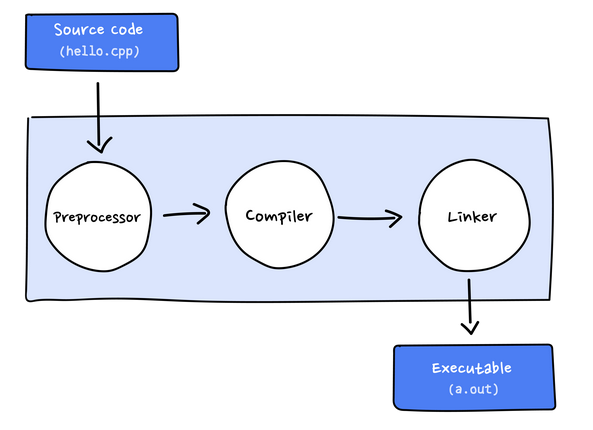
\includegraphics[width=3.5in]{compile.png}
\end{center}
\begin{center}
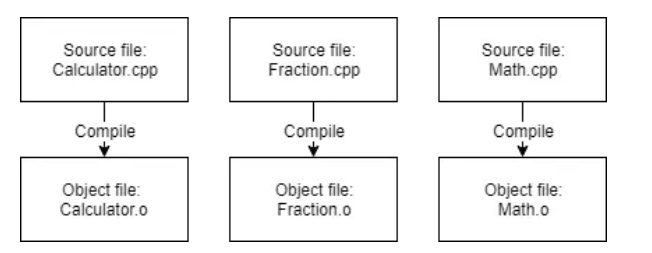
\includegraphics[width=3.5in]{compiling.png}
\end{center}

\begin{verbatim}
MVSC // Microsoft Compiler
GCC // Gnu C Compiler
LLVM Clang // LLVM Compiler
\end{verbatim}

\section{Linker}
\begin{verbatim}
    It combined all object files in one executable.
    the linker links library files. 
    resolves cross-file dependencies.  
\end{verbatim}

\begin{center}
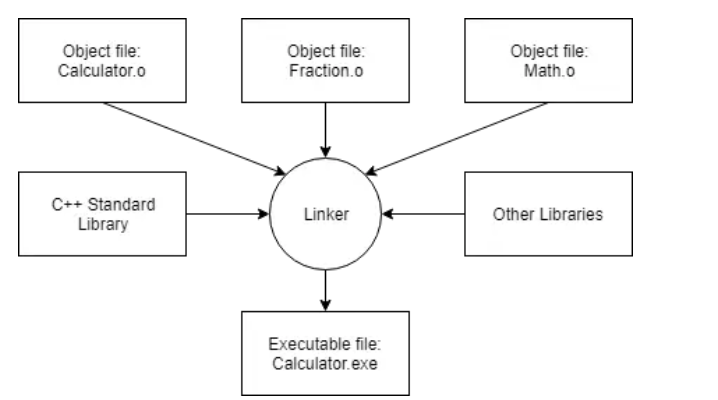
\includegraphics[width=2in]{linker.png}
\end{center}
\section{Libraries}
\subsection{Library files}
\begin{verbatim}
    a collection of precompiled code that has been "packaged up" for reuse in other programs. 
    C++ comes with a standard library providing additional functionality.
    commonly used in the iostream library
\end{verbatim}

\subsection{External Libraries}

A collection of pre-compiled code, providing functionality.

Functions, classes, and data structures that are not part of the standard C++ library.

These libraries are often provided by third-party developers or organizations

They speed up the development process by providing ready-to-use functionality. 

\begin{verbatim}
Popular C++ external libraries:
\end{verbatim}

\subsection{Boost}

\subsection{OpenCV}

\subsection{Qt}

\section{Builds}
\subsection{Build Configuration (build target)}

\begin{verbatim}
    Project settings determining how your project will be built. 
    Build configuration includes executable name, project arch and library files. 
    It specifies keepings or strippings of debugging info, compiler optimization details 
\end{verbatim}

\subsection{Debug Config}

\begin{verbatim}
    Debug configuations turns off all optimizations, includes debugging information,
    Jason Turner would say "with as much information as possible"
    Such configs makes your programs larger and slower, but much easier to debug. 
\end{verbatim}

\subsection{Release Config}

\begin{verbatim}
    Optimized for size and performance, no debugging information.
    With all optimization, now testing for code performance.

    When the Hello World program (from lesson 0.7) was built using Visual Studio,
    Executable produced in the debug configuration was 65kb, 
    Executable built in the release version was 12kb. 
    The difference is largely due to the extra debugging information kept in the debug build.
\end{verbatim}

\subsection{G++ Builds}
\begin{verbatim}
GCC / Clang? 
    -ggdb  // cmd line debugging
           // This is the GNU Debugger !?
    -ggdb O2 -DNDEBUG for release builds. ??
    -g++ O2 -DNDEBUG for release builds. ??
\end{verbatim}

\section{Compiler Extensions (compiler-specific behavior)}

    many compilers implement their own changes to the language,
    \begin{verbatim}
    Using compiler extension allows you to write programs that are incompatible
    with the C++ standard.
    \end{verbatim}

    Programs using non-standard extensions generally will not compile on other compilers (lacking same extensions support)
    , or if they do, they may not run correctly.

    Compiler extensions are often enabled by default. Overpermissive compilers.

    Compiler extensions are optional, cause programs non-compliancy with C++ standards,
    Turn compiler extensions off.

\begin{verbatim}
GCC
         -pedantic-errors // Disable extensions
\end{verbatim}

\section{Max Warnings}

\begin{verbatim}
GCC 
    -Wall -Weffc++ -Wextra -Wsign-conversion
    -Werror

Turner does it with cmake?
\end{verbatim}

\section{Standard Set-Up}

\begin{verbatim}
GCC pre-8
          -std=c++11 // set c++ standard
          -std=c++14
          -std=c++17
          -std=c++20 
GCC 8 or 9
          -std=c++2a for C++20 support

g++ -std=c++17 myfile.cpp -o output // cmd line
\end{verbatim}

\section{Dear ImGui}

\section{PCH - Precompiling Headers}

Some compilers' feature to speed compilation of large projects. 
It generates a precompiled version of commonly included header files, 

This version is known as the PCH file.
It is used during subsequent compilations. Avoids reparse and re-process of header files.

Great for large projects: numerous headers, included in multiple source files.

\subsection{Enable PCH}

PCH usage is compiler-specific, the enabling and configuring method varies. 

It typically involves specifying which headers should be precompiled and how the precompiled information should be stored.

\subsection{Include Header Files}

\begin{verbatim}
// Main.cpp
// #include "my_function.hpp"

//then
// g++ main.cpp my_function.cpp -o program
\end{verbatim}

\subsection{Header Files 2.0}

\begin{verbatim}
// Declare in header, fun.hpp or fun.h
double average(double num1, double num2);

// Define in fun.cpp
double average(double num1, double num2) {
  return (num1 + num2) / 2;
}
\end{verbatim}

\subsection{Standard Library Headers}

\begin{verbatim}
Some standard library headers are included by others. 

<cstdlib> is included by <iostream>, since it relies on its functionalities,
such as the declaration of the system() function. 
\end{verbatim}

\section{Command Line Linking and Compiling}

\begin{verbatim}
g++ main.cpp my_functions.cpp // link both files
\end{verbatim}

\subsection{Source Code Files Suffix}

\begin{verbatim}
    .cpp (ex: hello.cpp) or
    .h (ex: std_lib_facilities.h).
\end{verbatim}

\subsection{Compile}
\begin{verbatim}
g++ hello.cpp -o hello

Compiling translates C++ programs into machine code.
It is stored on disk as a file with the .o extension (hello.o). 
\end{verbatim}

A linker then links the object code with standard library routines that the program may use and creates an executable image which is also saved on disk,

usually as a file with the file name without any extension (e.g. hello).

\section{Debugg and Error Type}

\subsection{Compile Time Errors}

\subsection{Synthax Errors}

\subsection{Type errors}

Forgetting to declare a variable

Storing a value in a different type. 

\subsection{Link-Time Errors}

link-time errors are based on unfindable needed function or library.

When the linker tries to combine object files into an executable.

\subsection{Run-Time Errors}

Errors which happen during program execution (run-time) after successful compilation.

Division by zero

Open an non-existing file

\subsection{Logical Errors}

Flawed programming's logical thinking. 

No errors, but output is wrong. 


\chapter{Filesystem Libray}

LOOK AT FILESYSTEM VIDEO IN CODE

Introduced in c++17, the language has a filesystem library allowing
manipulation of paths, regular files and directories.

\section{Files}

\subsection{File Creation}

Use the fstream header and the ofstream function.

\begin{verbatim}
#include <filesystem>
#include <iostream>
#include <fstream> // Add this header for std::ofstream
namespace fs = std::filesystem;

int main() {
    fs::create_directories("sandbox/a");

    std::ofstream("sandbox/file.1.txt");     // is simplest,

    std::ofstream file("sandbox/file1.txt"); // initialize the variable on top!

    // Check if the file was opened successfully
    if (file.is_open()) {

        file << "This is some content written to the file.\n";

        file.close(); // Close the file after writing if no longer needed

    } else {
        std::cout << "Failed to open the file.\n";
    }

    return 0;
}
\end{verbatim}


\subsection{File Deletion}

\section{Paths}

\section{Directories}

\subsection{Directory Creation}

Create a directory with fs::create\_directories. This creates both sandbox and a, inside it.

\begin{verbatim}
#include <filesystem>
namespace fs = std::filesystem;

int main() {

    fs::create_directories("sandbox/a");
    std::ofstream("sandbox/file1.txt");
    std::ofstream("sandbox/file2.txt");

    for (auto& p : fs::directory_iterator("sandbox")) {
        std::cout << p.path() << '\n';
    } 

fs::remove_all("sandbox");

}
\end{verbatim}


\subsection{File Creation}



\subsection{Testing Framework}

\section{Benchmarking strategy}
\subsection{Chrono, clock time}

\begin{verbatim}
#include <chrono>
int main() {

  // Measure time taken for goodnight1():
  std::chrono::high_resolution_clock::time_point start = std::chrono::high_resolution_clock::now();

  std::cout << goodnight1("tulip");

  std::chrono::high_resolution_clock::time_point end = std::chrono::high_resolution_clock::now();
  std::chrono::duration<double, std::milli> time_span = end - start;

  // Print time taken for goodnight1():
  std::cout << "Time taken for goodnight1(): " << time_span.count() << " milliseconds.\n\n";
\end{verbatim}

\section{Good practices}

\subsection{Proper Design}

\begin{verbatim}
    if a component is hard to test, it is not properly designed. 
    if a component is easy to test, it indicates proper design. 
    Approval tests ressource : https://cppcast.com/clare-macrae/ 
\end{verbatim}

\subsection{Warnings}

Enable as many compiler warnings as you can. 
Fix new warning generated. 

\textbf{It will feel tedious and meaningfless}
\textbf{But this is the c++ way to catch real bugs.}

\subsection{Slow Down!}

\begin{verbatim}
Copy and pasting is easy. 
Forging ahead in comfort is too easy.
Plan ahead, don't get caught off guard. 
\end{verbatim}

\subsection{Ponder for solutions}

\begin{verbatim}
If the solution seems large or complex, stop. 
Walk and ponder for the solution. 
discuss the design with a rubber duck. 
spend less time programming, more thinking.
\end{verbatim}

\subsection{C++ is not magic nor Object-Oriented}

\begin{verbatim}
It's not magic, construct to test your doubts.
It is multi-disciplinary, supports all programming paradigms.

    Procedural
    Functional
    Object-Oriented
    Generic
    Compile-Time(contexpr and template metaprogramming)

Knowing when paradims are needed is the key to good C++.
Using appropriate techniques takes time and appropriate technique. 
\end{verbatim}

\subsection{Learn a different language}

\begin{verbatim}
    Lisp // Diverge from the C-family languages. Learn,
    Haskell
    Erlang
\end{verbatim}

